\section{CARGAR}
\subsection{Gráfico de dependencias}
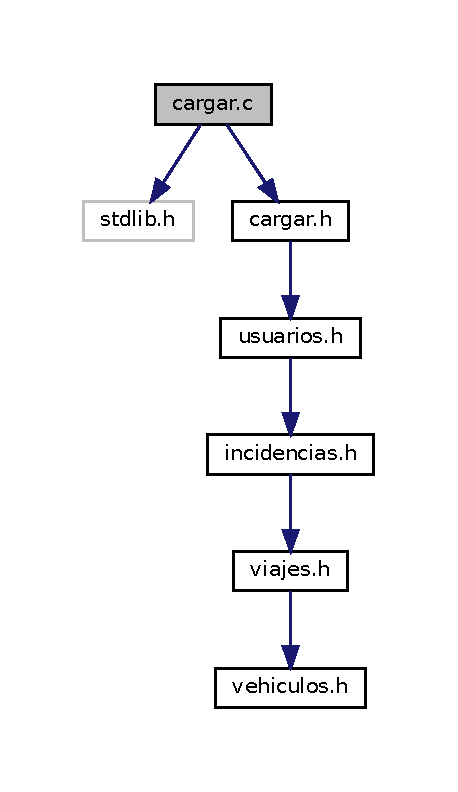
\includegraphics[width=\textwidth, angle=0,scale=0.4]{dep/cargar_include.pdf}
\subsection{Funciones}
\begin{itemize}
    \item \cc{void init(vUsuarios* vu,vIncidencias* vi,vViajes* vv,vVehiculos* vve)}
    \item \cc{void save(vUsuarios* vu,vIncidencias* vi,vViajes* vv,vVehiculos* vve)}
\end{itemize}
\subsection{Definiciones}
\begin{itemize}
     \item \cc{void init(vUsuarios* vu,vIncidencias* vi,vViajes* vv,vVehiculos* vve)}
    \begin{itemize}
        \item \textbf{Descripción}
        \begin{itemize}
			\item Inicializa los vectores de usuarios, incidencias, viajes y vehiculos.
		\end{itemize}
		\item \textbf{Parámetros}
		\begin{itemize}
			\item \cc{v} $\rightarrow$ Referencia al vector user.
			\item \cc{vi} $\rightarrow$ Referencia al vector inci.
			\item \cc{vv} $\rightarrow$ Referencia al vector viajes.
			\item \cc{vve} $\rightarrow$ Referencia al vector vehi.
		\end{itemize}
	\end{itemize}
    \item \cc{void save(vUsuarios* vu,vIncidencias* vi,vViajes* vv,vVehiculos* vve)}
    \begin{itemize}
        \item \textbf{Descripción}
        \begin{itemize}
			\item Guarda datos de usuarios, incidencias, viajes y vehiculos en ficheros y libera memoria.
		\end{itemize}
		\item \textbf{Parámetros}
		\begin{itemize}
			\item \cc{v} $\rightarrow$ Referencia al vector user.
			\item \cc{vi} $\rightarrow$ Referencia al vector inci.
			\item \cc{vv} $\rightarrow$ Referencia al vector viajes.
			\item \cc{vve} $\rightarrow$ Referencia al vector vehi.
		\end{itemize}
	\end{itemize}
\end{itemize}
\newpage
